\section{Discussão}

    % Aqui deve ser discutido o problema tratado pelo trabalho, de modo fundamentado,
    % com citações diretas e indiretas. Essa discussão deve ser feita de modo que
    % contenha informações suficientes para o desenvolvimento do objetivo de trabalho.
    Abaixo será discutido e analisado o que pode ser feito para diminuir a alta taxa de
    roubos de celulares por assaltantes disfarçados de motoqueiros no Grajaú, baseando-se
    em estatísticas e notícias deste e de outros bairros em situações semelhantes da cidade
    de São Paulo.

    Esta seção foi separada em três tópicos: Origem, Dados e estatísticas e Sugestões de melhora.

    \subsection{Origem}

        Com a flexibilização da quarentena devido ao Covid-19 e a popularização de aplicativos
        e serviços de entrega de alimentos, os casos de assaltos envolvendo assaltantes 
        disfarçando-se de entregadores de aplicativos começaram a aumentar 
        
        Devido à sua valorização, uma das coisas que os assaltantes mais procuram roubar é o
        celular, pois além de seu preço, é fácil de ser transportado e quando a vítima está
        distraída com ele, torna-se ainda mais fácil de realizar o assalto.
        
        Outro fator que faz o celular ser prioridade dos assaltantes é que caso o assaltante
        consiga roubar o celular enquanto ele está desbloqueado, o assaltante terá 
        acesso direto as informações pessoais do dono do celular, como os contatos e redes 
        sociais, mas também poderá usufruir de funções como utilizar o cartão de crédito que 
        normalmente fica armazenado no celular.

        Além da facilidade de ser transportado e de ser um produto muito valorizado, há também a
        baixa penalidade para quem rouba, para furtos a penalidade é de 1 a 4 anos de reclusão e 
        multa, e para assaltos é de 4 a 10 anos além da multa.

    \subsection{Dados e estatísticas}

        \subsubsection{Com que frequência ocorrem os roubos}
        Segundo a notícia feita pelo programa jornalístico SP1 e publicada no site G1 - Globo,
        no dia 19 de Maio de 2022, foram em todo o estado 26.484 furtos nos dois primeiros 
        meses do ano e 34.338 roubos no mesmo período, de acordo com dados dos boletins de 
        ocorrência. Este levantamento foi feito pela GloboNews. A notícia também apresenta que
        a cada hora 42 celulares são furtados ou roubados no estado de São Paulo. Grande parte
        das vítimas deste tipo de crime são pedestres no período da noite na cidade de São Paulo.
        Na capital, encontra-se o Grajaú como um dos bairros que possui os maiores números de ocorrências.

        O programa jornalístico também informa sobre um pacote de medidas preventivas
        do governo do estado de São Paulo, com o intuito de inibir a onda de ocorrências
        envolvendo assaltantes disfarçados de entregadores de aplicativos, realizando mais
        abordagens aos motociclistas e parcerias às empresas dos respectivos aplicativos para
        uma fiscalização mais efetiva.
        % https://g1.globo.com/sp/sao-paulo/noticia/2022/05/19/42-celulares-sao-roubados-ou-furtados-por-hora-no-estado-de-sp-em-janeiro-e-fevereiro.ghtml
        % Data 19 de Maio, 2022
        % Título: 42 Celulares são roubados ou furtados por hora no estado de São Paulo em Janeiro e Fevereiro
        % Autor: G1 - Globo, SP1 (Eu acho)

        \subsubsection{Onde se concentram os roubos}
        Há dados sobre onde mais se concentram os roubos de celulares no estado de São 
        Paulo no jornal Folha de São Paulo. Segundo os escritores Alfredo Henrique e William
        Cardoso, a volta do trabalho no início da noite é o horário no qual se corre o maior
        risco de ter o celular roubado na capital paulista, o perigo é maior para os moradores
        das periferias, onde estão os bairros que lideram nesse tipos de crime.

        Um levantamento feito pela reportagem analisou que foram registrados mais de 89.000
        boletins de ocorrência em 2021, constatando que no período entre 19h e 21h59 concentra
        1 em cada 4 roubos de celular (26,5\% das ocorrências).
        
        Na zona sul de São Paulo, bairros como Capão Redondo, Campo Limpo, Jardim Ângela,
        Jardim São Luís, e inclusive o Grajaú, onde ficam 6 dos 10 distritos policiais com
        mais assaltos em que celulares foram roubados, são as regiões com maior incidência
        do crime.

        \begin{figure}[H]
            \centering
            \textbf{Mapa dos Roubos de Celular em São Paulo}
            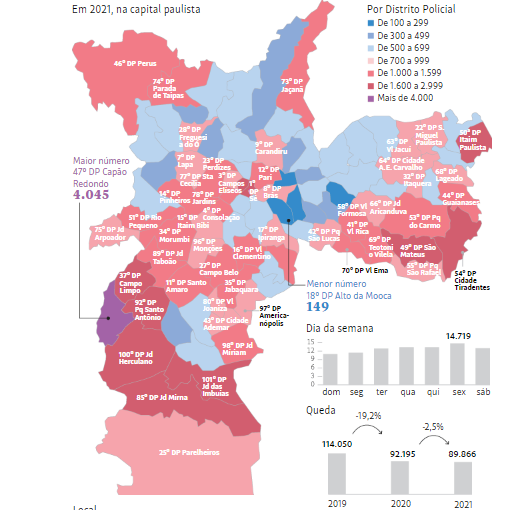
\includegraphics[scale=0.7]{img/mapa_dos_roubos_de_celular_em_sp.png}
            \caption{Fonte: Gráfico feito pela Folha S. Paulo, com dados da Secretaria da Segurança Pública do Estado de São Paulo}
        \end{figure}

        Observando os dados gerais, os casos de roubos de celular na capital paulista caíram
        de 114.050 para 92.195, entre 2019 e 2020, e para 89.866 em 2021. É possível observar
        também que grande parte dos roubos ocorrem na zona sul de São Paulo em relação às
        outras regiões da capital.
        % https://www1.folha.uol.com.br/cotidiano/2022/02/roubo-de-celular-se-concentra-na-volta-para-casa-e-na-periferia-de-sp.shtml
        % Data: 25 fev. 2022
        % Autores: Alfredo Henrique, William Cardoso
        % Título: Roubo de celular se concentra na volta para casa e na periferia de SP

    \subsection{Sugestões de melhora}

        De acordo com um especialista em segurança citado pelo programa jornalístico SP1, no dia 
        19 de Maio de 2022, há diversas coisas que podemos fazer para se proteger em caso de
        roubo de celular. "A primeira e mais simples é a senha. Não podem ser fáceis, dedutíveis
        ou estarem anotadas no celular. O que tem acontecido é roubo de celular quando ele está
        desbloqueado, seja por motoristas presos no celular ou pedestres utilizando-o na mão. O
        telefone na mão já é a primeira barreira derrubada, permitindo que os bandidos acessem
        nossos dados e até contas bancárias. Também todos nós devemos estar preparados para este 
        acidente. Quais são os telefones dos bancos que você tem de ligar? No momento de nervosismo,
        é importante ter esse roteiro na bolsa, no porta-luvas do carro, em casa, para você chegar
        e poder avisar que foi roubado.", o especialista afirma.
        % https://g1.globo.com/sp/sao-paulo/noticia/2022/05/19/42-celulares-sao-roubados-ou-furtados-por-hora-no-estado-de-sp-em-janeiro-e-fevereiro.ghtml

        Como sugestão de melhora, é possível realizar uma regularização para entregadores de
        aplicativo e aumentar as patrulhas policiais, evitando a possibilidade de assaltantes 
        se disfarçarem e facilitando a fiscalização para as autoridades. Alguns exemplos de 
        fiscalização que podem ser feitas são nos registros dos entregadores nos aplicativos, 
        dando mais recursos para poder distinguir entre quem está trabalhando e quem está se 
        disfarçando para diminuir suspeitas. Além disso o que pode ser feito é dar uma 
        formalização ao trabalho de entregador de aplicativo, possibilitando até mesmo a 
        utilização da placa para serviços e aluguéis ao invés da placa para veículos particulares.
